%!TEX TS-program = xelatex
\documentclass[10pt,oneside]{article}

\usepackage[english]{babel}

\usepackage{amsmath,amssymb,amsfonts}
\usepackage[utf8]{inputenc}
\usepackage[T1]{fontenc}
\usepackage{stix}
\usepackage[scaled]{helvet}
\usepackage[scaled]{inconsolata}

\usepackage{lastpage}

\usepackage{setspace}

\usepackage{ccicons}

\usepackage[hang,flushmargin]{footmisc}

\usepackage{geometry}

\setlength{\parindent}{0pt}
\setlength{\parskip}{6pt plus 2pt minus 1pt}

\usepackage{fancyhdr}
\renewcommand{\headrulewidth}{0pt}\providecommand{\tightlist}{%
  \setlength{\itemsep}{0pt}\setlength{\parskip}{0pt}}

\makeatletter
\newcounter{tableno}
\newenvironment{tablenos:no-prefix-table-caption}{
  \caption@ifcompatibility{}{
    \let\oldthetable\thetable
    \let\oldtheHtable\theHtable
    \renewcommand{\thetable}{tableno:\thetableno}
    \renewcommand{\theHtable}{tableno:\thetableno}
    \stepcounter{tableno}
    \captionsetup{labelformat=empty}
  }
}{
  \caption@ifcompatibility{}{
    \captionsetup{labelformat=default}
    \let\thetable\oldthetable
    \let\theHtable\oldtheHtable
    \addtocounter{table}{-1}
  }
}
\makeatother

\usepackage{array}
\newcommand{\PreserveBackslash}[1]{\let\temp=\\#1\let\\=\temp}
\let\PBS=\PreserveBackslash

\usepackage[breaklinks=true]{hyperref}
\hypersetup{colorlinks,%
citecolor=blue,%
filecolor=blue,%
linkcolor=blue,%
urlcolor=blue}
\usepackage{url}

\usepackage{caption}
\setcounter{secnumdepth}{0}
\usepackage{cleveref}

\usepackage{graphicx}
\makeatletter
\def\maxwidth{\ifdim\Gin@nat@width>\linewidth\linewidth
\else\Gin@nat@width\fi}
\makeatother
\let\Oldincludegraphics\includegraphics
\renewcommand{\includegraphics}[1]{\Oldincludegraphics[width=\maxwidth]{#1}}

\usepackage{longtable}
\usepackage{booktabs}

\usepackage{color}
\usepackage{fancyvrb}
\newcommand{\VerbBar}{|}
\newcommand{\VERB}{\Verb[commandchars=\\\{\}]}
\DefineVerbatimEnvironment{Highlighting}{Verbatim}{commandchars=\\\{\}}
% Add ',fontsize=\small' for more characters per line
\usepackage{framed}
\definecolor{shadecolor}{RGB}{248,248,248}
\newenvironment{Shaded}{\begin{snugshade}}{\end{snugshade}}
\newcommand{\KeywordTok}[1]{\textcolor[rgb]{0.13,0.29,0.53}{\textbf{#1}}}
\newcommand{\DataTypeTok}[1]{\textcolor[rgb]{0.13,0.29,0.53}{#1}}
\newcommand{\DecValTok}[1]{\textcolor[rgb]{0.00,0.00,0.81}{#1}}
\newcommand{\BaseNTok}[1]{\textcolor[rgb]{0.00,0.00,0.81}{#1}}
\newcommand{\FloatTok}[1]{\textcolor[rgb]{0.00,0.00,0.81}{#1}}
\newcommand{\ConstantTok}[1]{\textcolor[rgb]{0.00,0.00,0.00}{#1}}
\newcommand{\CharTok}[1]{\textcolor[rgb]{0.31,0.60,0.02}{#1}}
\newcommand{\SpecialCharTok}[1]{\textcolor[rgb]{0.00,0.00,0.00}{#1}}
\newcommand{\StringTok}[1]{\textcolor[rgb]{0.31,0.60,0.02}{#1}}
\newcommand{\VerbatimStringTok}[1]{\textcolor[rgb]{0.31,0.60,0.02}{#1}}
\newcommand{\SpecialStringTok}[1]{\textcolor[rgb]{0.31,0.60,0.02}{#1}}
\newcommand{\ImportTok}[1]{#1}
\newcommand{\CommentTok}[1]{\textcolor[rgb]{0.56,0.35,0.01}{\textit{#1}}}
\newcommand{\DocumentationTok}[1]{\textcolor[rgb]{0.56,0.35,0.01}{\textbf{\textit{#1}}}}
\newcommand{\AnnotationTok}[1]{\textcolor[rgb]{0.56,0.35,0.01}{\textbf{\textit{#1}}}}
\newcommand{\CommentVarTok}[1]{\textcolor[rgb]{0.56,0.35,0.01}{\textbf{\textit{#1}}}}
\newcommand{\OtherTok}[1]{\textcolor[rgb]{0.56,0.35,0.01}{#1}}
\newcommand{\FunctionTok}[1]{\textcolor[rgb]{0.00,0.00,0.00}{#1}}
\newcommand{\VariableTok}[1]{\textcolor[rgb]{0.00,0.00,0.00}{#1}}
\newcommand{\ControlFlowTok}[1]{\textcolor[rgb]{0.13,0.29,0.53}{\textbf{#1}}}
\newcommand{\OperatorTok}[1]{\textcolor[rgb]{0.81,0.36,0.00}{\textbf{#1}}}
\newcommand{\BuiltInTok}[1]{#1}
\newcommand{\ExtensionTok}[1]{#1}
\newcommand{\PreprocessorTok}[1]{\textcolor[rgb]{0.56,0.35,0.01}{\textit{#1}}}
\newcommand{\AttributeTok}[1]{\textcolor[rgb]{0.77,0.63,0.00}{#1}}
\newcommand{\RegionMarkerTok}[1]{#1}
\newcommand{\InformationTok}[1]{\textcolor[rgb]{0.56,0.35,0.01}{\textbf{\textit{#1}}}}
\newcommand{\WarningTok}[1]{\textcolor[rgb]{0.56,0.35,0.01}{\textbf{\textit{#1}}}}
\newcommand{\AlertTok}[1]{\textcolor[rgb]{0.94,0.16,0.16}{#1}}
\newcommand{\ErrorTok}[1]{\textcolor[rgb]{0.64,0.00,0.00}{\textbf{#1}}}
\newcommand{\NormalTok}[1]{#1}

\newlength{\cslhangindent}
\setlength{\cslhangindent}{1.5em}
\newlength{\csllabelwidth}
\setlength{\csllabelwidth}{3em}
\newenvironment{CSLReferences}[3] % #1 hanging-ident, #2 entry spacing
 {% don't indent paragraphs
  \setlength{\parindent}{0pt}
  % turn on hanging indent if param 1 is 1
  \ifodd #1 \everypar{\setlength{\hangindent}{\cslhangindent}}\ignorespaces\fi
  % set entry spacing
  \ifnum #2 > 0
  \setlength{\parskip}{#2\baselineskip}
  \fi
 }%
 {}
\usepackage{calc} % for \widthof, \maxof
\newcommand{\CSLBlock}[1]{#1\hfill\break}
\newcommand{\CSLLeftMargin}[1]{\parbox[t]{\maxof{\widthof{#1}}{\csllabelwidth}}{#1}}
\newcommand{\CSLRightInline}[1]{\parbox[t]{\linewidth}{#1}}
\newcommand{\CSLIndent}[1]{\hspace{\cslhangindent}#1}\usepackage[table,dvipsnames]{xcolor}

\geometry{includemp,
            letterpaper,
            top=1.2in,
            bottom=2.510cm,
            inner=0.5in,
            outer=0.4in,
            marginparwidth=1.95in,
            marginparsep=0.4in}

\usepackage[singlelinecheck=off]{caption}
\captionsetup{
  font={small},
  labelfont={bf},
  format=plain,
  labelsep=quad
}
\usepackage{floatrow}
\floatsetup[figure]{margins=hangright,
              facing=no,
              capposition=beside,
              capbesideposition={center,outside},
              floatwidth=\textwidth}
\floatsetup[table]{margins=hangoutside,
             facing=yes,
             capposition=beside,
             capbesideposition={center,outside},
             floatwidth=\textwidth}

\pagestyle{plain}

\setcounter{secnumdepth}{5}

\usepackage{titlesec}

\titleformat{\section}[block]
{\normalfont\large\sffamily}
{\thesection}{.5em}{\titlerule\\[.8ex]\bfseries}

\titleformat{\subsection}[runin]
{\normalfont\fontseries{b}\selectfont\filright\sffamily}
{\thesubsection.}{.5em}{}

\titleformat{\subsubsection}[runin]
{\normalfont\itshape\rmfamily\bfseries}{\thesubsubsection}{1em}{}

\fancypagestyle{firstpage}
{
   \fancyhf{}
   \renewcommand{\headrulewidth}{0pt}
   \fancyfoot[R]{\footnotesize\ccby}
   \fancyfoot[L]{\footnotesize\sffamily\today}
}

\fancypagestyle{normal}
{
  \fancyhf{}
  \fancyfoot[R]{\footnotesize\sffamily\thepage\ of \pageref*{LastPage}}
}

\usepackage{tikz}
\begin{document}
\tikz [remember picture, overlay] %
\node [shift={(-0.6in,1.1cm)},scale=0.2,opacity=0.4] at (current page.south east)[anchor=south east]{
\includegraphics{logo}};%
\pagestyle{normal}
\thispagestyle{firstpage}

\newcommand{\colorRule}[3][black]{\textcolor[HTML]{#1}{\rule{#2}{#3}}}

\noindent {\LARGE \textbf{\textsf{Preprint template}}}

\medskip
\begin{flushleft}
{\small
%
\href{https://orcid.org/0000-0002-6506-6487}{M.D.\,Catchen}%
%
\,\textsuperscript{1,2}
\vskip 1em
\textsuperscript{1}\,McGill University; \textsuperscript{2}\,Québec
Centre for Biodiversity Sciences\\
\vskip 1em
\textbf{Correspondance to:}\\
}
\end{flushleft}

\vskip 2em
\makebox[0pt][l]{\colorRule[CCCCCC]{2.0\textwidth}{0.5pt}}
\vskip 2em
\noindent

\marginpar{\vskip 1em\flushright
{\small{\bfseries Keywords}:\par
pandoc\\pandoc-crossref\\github actions\\}
}


\textbf{Abstract}:\,This template is used by the Poisot lab at
Université de Montréal to write manuscripts using github. It uses github
actions as a way to generate a website that can be annotated using
hypothes.is, a PDF document for copy-editing and submission to journals,
and a PDF document for submission to preprint servers. At every push on
the master branch, the whole series of documents will be updated
automatically.

\vskip 2em
\makebox[0pt][l]{\colorRule[CCCCCC]{2.0\textwidth}{0.5pt}}
\vskip 2em

This template uses recent versions of \texttt{pandoc} and
\texttt{pandoc-crossref} to facilitate the referencing of equations,
figures, and tables within the text. For example, the following equation

\begin{equation}\protect\hypertarget{eq:eq1}{}{J'(p) = \frac{1}{\text{log}(S)}\times\left(-\sum p \times \text{log}(p)\right)}\label{eq:eq1}\end{equation}

is produced using

\begin{Shaded}
\begin{Highlighting}[]
\SpecialStringTok{$$J\textquotesingle{}(p) = }\SpecialCharTok{\textbackslash{}frac}\SpecialStringTok{\{1\}\{}\SpecialCharTok{\textbackslash{}text}\NormalTok{\{log\}}\SpecialStringTok{(S)\}}\SpecialCharTok{\textbackslash{}times\textbackslash{}left}\SpecialStringTok{({-}}\SpecialCharTok{\textbackslash{}sum}\SpecialStringTok{ p }\SpecialCharTok{\textbackslash{}times}\SpecialStringTok{ }\SpecialCharTok{\textbackslash{}text}\NormalTok{\{log\}}\SpecialStringTok{(p)}\SpecialCharTok{\textbackslash{}right}\SpecialStringTok{)$$}\NormalTok{ \{\#eq:eq1\}}
\end{Highlighting}
\end{Shaded}

and can be referenced using \texttt{@eq:eq1}, which will result in
eq.~\ref{eq:eq1}.

All documents will be deployed to \texttt{gh-pages} \emph{only} on push
events from the \texttt{master} branch. All of the artifacts will be
built when doing pull requests, so you can check that merging a branch
is \emph{not} going to cause the compilation of the documents to fail;
indeed, you can download the artifacts produced during the run, to check
the PDF and html files.

\hypertarget{using-references}{%
\section{Using references}\label{using-references}}

The references are managed by \texttt{pandoc}. Note that we \emph{do
not} use \texttt{pandoc-citeproc}, which was an external module for
older \texttt{pandoc} versions. References \emph{must} be stored in a
\texttt{references.bib} file. We use
\href{https://www.zotero.org/}{Zotero} for references management, and
for the lab's manuscripts, we work from folders in a shared library
(with a folder for every manuscript).

We use the \href{https://retorque.re/zotero-better-bibtex/}{Better
BibTeX} plugin for citation key generations, and auto-export of the
shared library to the \texttt{references.bib} file. We use a citation
key format meant to convey information on the author, date, year, and
title. It must be set in the Better BibTeX preferences as

\begin{verbatim}
[auth:fold][year][title:fold:nopunctordash:skipwords:lower:select=1,1:substring=1,3:capitalize][title:fold:nopunctordash:skipwords:lower:select=2,2:substring=1,3:capitalize]
\end{verbatim}

It is a good idea to configure Better BibTeX to auto-export on change,
and to remove a lot of fields that are not strictly speaking required
for references. The list of fields we usually ignore is:

\begin{verbatim}
abstract,copyright,annotation,file,pmid,month,shorttitle,keywords
\end{verbatim}

The citations are done using the normal markdown syntax, where
\texttt{@Elton1927AniEco} produces Elton (1927), and
\texttt{{[}@Camerano1880EquViv{]}} produces (Camerano 1880).

\hypertarget{tables}{%
\section{Tables}\label{tables}}

Table legends go on the line after the table itself. To generate a
reference to the table, use \texttt{\{\#tbl:id\}} -- then, in the text,
you can use \texttt{\{@tbl:id\}} to refer to the table. For example, the
table below is tbl.~\ref{tbl:id}. You can remove the \emph{table} in
front by using \texttt{!@tbl:id}, or force it to be capitalized with
\texttt{\textbackslash{}*tbl:id}.

\hypertarget{tbl:id}{}
\begin{longtable}[]{@{}rrrrl@{}}
\caption{\label{tbl:id}This is a table, and its identifier is
\texttt{id} -- we can refer to it using \texttt{\{@tbl:id\}}. Note that
even if the table legend is written below the table itself, it will
appear on top in the PDF document.}\tabularnewline
\toprule
Sepal.Length & Sepal.Width & Petal.Length & Petal.Width &
Species\tabularnewline
\midrule
\endfirsthead
\toprule
Sepal.Length & Sepal.Width & Petal.Length & Petal.Width &
Species\tabularnewline
\midrule
\endhead
5.1 & 3.5 & 1.4 & 0.2 & setosa\tabularnewline
5.0 & 3.6 & 1.4 & 0.2 & setosa\tabularnewline
5.4 & 3.9 & 1.7 & 0.4 & setosa\tabularnewline
\bottomrule
\end{longtable}

\hypertarget{figures}{%
\section{Figures}\label{figures}}

Figures can have a legend -- all figures \emph{must} be in the
\texttt{figures/} folder of the project, as it is also used for the
website. We recommend to use good resolution images, rather than PDFs,
or at least to have multiple versions available.

\begin{verbatim}
![This is the legend of the figure](figures/biomes.png){#fig:biomes}
\end{verbatim}

\begin{figure}
\hypertarget{fig:biomes}{%
\centering
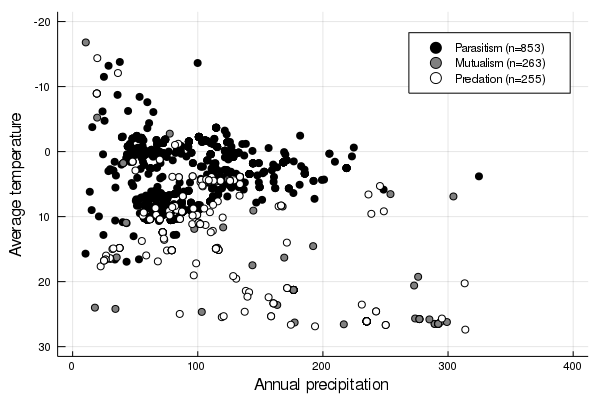
\includegraphics{figures/biomes.png}
\caption{This is the legend of the figure}\label{fig:biomes}
}
\end{figure}

We can now use \texttt{@fig:biomes} to refer to fig.~\ref{fig:biomes}.

\hypertarget{example-text}{%
\section{Example text}\label{example-text}}

Connectance, defined as the ratio of realized interactions on the total
number of potential interactions, is one of the most common descriptor
of network structure. In a bipartite network with \(T\) species at the
top, and \(B\) at the bottom, having a total of \(L\) interactions, it
is defined as \(Co = L/(T\times B)\). Connectance has a lower bound, as
the network cannot have fewer interactions that the number of species in
its more speciose level -- the minimal connectance is therefore
\(c_m = \text{max}(T,B)\). This makes the connectance of networks of
different sizes difficult to compare, especially since bipartite
networks tends to have a low connectance. For this reason, we used a
corrected version of connectance, defined as

\begin{equation}\protect\hypertarget{eq:cstar}{}{Co^\star=\frac{L-c_m}{T\times B-c_m} \,.}\label{eq:cstar}\end{equation}

\hypertarget{this-is-a-subsection}{%
\subsection{This is a subsection}\label{this-is-a-subsection}}

This takes values between 0 (the network has the minimal number of
interactions) and 1 (all species are connected), but is robust to
variations in species richness.

\hypertarget{this-is-another-subsection}{%
\subsection{This is another
subsection}\label{this-is-another-subsection}}

This takes values between 0 (the network has the minimal number of
interactions) and 1 (all species are connected), but is robust to
variations in species richness.

\hypertarget{references}{%
\section*{References}\label{references}}
\addcontentsline{toc}{section}{References}

\hypertarget{refs}{}
\begin{CSLReferences}{1}{0}
\leavevmode\hypertarget{ref-Camerano1880EquViv}{}%
Camerano, Lorenzo. 1880. {``Dell'equilibrio Dei Viventi Merce La
Reciproca Distruzione.''} \emph{Atti Della R. Accad. Delle Sci. Torino}
15: 393--414.

\leavevmode\hypertarget{ref-Elton1927AniEco}{}%
Elton, Charles S. 1927. \emph{Animal Ecology}. University of Chicago
Press.

\end{CSLReferences}

\end{document}
